\documentclass[border=3.14mm, tikz]{standalone}
\usetikzlibrary{3d,intersections}
\begin{document}

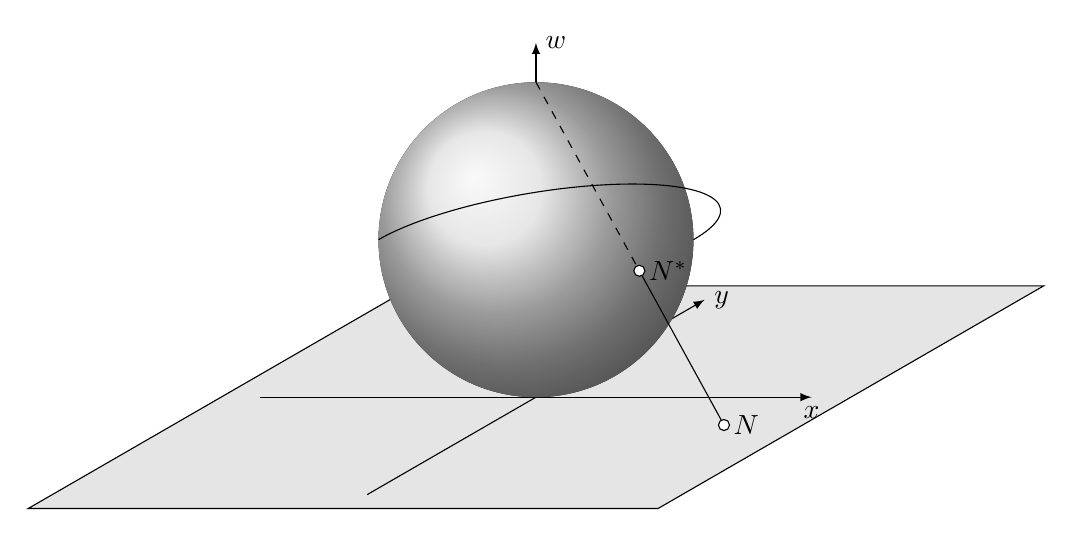
\begin{tikzpicture}[y={({(cos(30)/sqrt(2))*1cm},{(sin(30)/sqrt(2))*1cm})},x={(1cm,0cm)}, z={(0cm,1cm)},font=\sffamily]
\begin{scope}[canvas is xy plane at z=0]
\draw[fill=gray!20] (-4,-4) -- (4,-4) -- (4,4) -- (-4,4) -- cycle;
\end{scope}
\draw[-latex] (-3.5,0,0) -- (3.5,0,0) node[below]{$x$};
\draw[-latex] (0,-3.5,0) -- (0,3.5,0) node[right]{$y$};
\draw[-latex] (0,0,0) -- (0,0,4.5) node[right]{$w$};
\begin{scope}[canvas is xz plane at y=0]
\fill[ball color=white] (0,2) circle (2);
\shade[ball color=gray,opacity=0.25,name path global=circle] (0,2) circle(2);
\end{scope}
\path(0,0,4)--(3,-1,0)coordinate[pos=0.55](kA);
\draw[dashed](0,0,4)--(kA);
\draw(kA)--(3,-1,0);
\draw[fill=white](3,-1,0) circle (2pt)node[right]{$N$};
\draw[fill=white](kA) circle (2pt)node[right]{$N^*$};
\draw ([shift={(0:2)}]0,0,2) arc (0:180:2);
\end{tikzpicture}
\end{document}
